% Source-relative PDF page 1, Q18 (printed page 302).
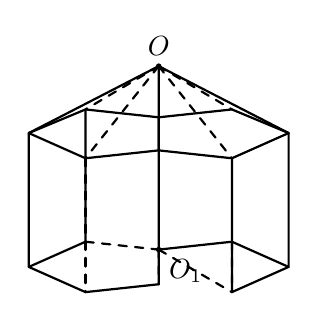
\begin{tikzpicture}[line cap=round,line join=round,thick]
  % Upper hexagonal pyramid, joined to a hexagonal prism below.
  \coordinate (O) at (1.65,3.65);
  \coordinate (A) at (0,2.8); \coordinate (B) at (0.72,3.1);
  \coordinate (C) at (1.65,3.0); \coordinate (D) at (2.58,3.1);
  \coordinate (E) at (3.3,2.8); \coordinate (F) at (2.58,2.48);
  \coordinate (G) at (1.65,2.58); \coordinate (H) at (0.72,2.48);
  \coordinate (I) at (0,1.1); \coordinate (J) at (0.72,1.42);
  \coordinate (K) at (1.65,1.32); \coordinate (L) at (2.58,1.42);
  \coordinate (M) at (3.3,1.1); \coordinate (N) at (2.58,0.78);
  \coordinate (Q) at (1.65,0.88); \coordinate (R) at (0.72,0.78);
  \draw (A)--(B)--(C)--(D)--(E) (E)--(F)--(G)--(H)--(A);
  \draw (O)--(A) (O)--(C) (O)--(E) (O)--(G);
  \draw[dashed] (O)--(B) (O)--(D) (O)--(F) (O)--(H);
  \draw (A)--(I)--(J)--(B) (C)--(K)--(G) (E)--(M)--(N)--(F);
  \draw (I)--(R)--(Q)--(K)--(L)--(M);
  \draw[dashed] (J)--(K) (J)--(R) (K)--(Q) (K)--(N) (L)--(N);
  \draw[dashed] (H)--(R) (G)--(Q) (F)--(N);
  \fill (O) circle (1pt) node[above] {$O$};
  \fill (K) circle (1pt) node[below right] {$O_1$};
\end{tikzpicture}
